\documentclass{article}
\usepackage[utf8]{inputenc}
\usepackage{gensymb}
\usepackage{hyperref}
\hypersetup{colorlinks=true,urlcolor=blue}
\usepackage{natbib}
\usepackage{graphicx}
\usepackage{indentfirst}
\usepackage{verbatim}
\usepackage{listings}
\usepackage[verbose]{wrapfig}
\usepackage{environ}
\usepackage{lipsum}
\lstset{
basicstyle=\small\ttfamily,
columns=flexible,
breaklines=true
}
%\usepackage[tikz]{bclogo}
\usepackage{marginnote}
\usepackage{graphicx}
\usepackage{pdflscape}
%\usepackage[paper=portrait,pagesize]{typearea}
\usepackage[T1]{fontenc}

\begin{document}
\begin{titlepage}
  \begin{figure}[t]
    \centering
    
\includegraphics[]{Figuras/00_unr.png}
    \hspace{0.15\textwidth}
    
\includegraphics[width=0.4\textwidth]{Figuras/00_eim.png}
\end{figure}
  
\begin{center}
    {\Huge Informe N\degree1:\\ Estudio de un caso RTD \par}
    
    %\date{November 2019}
    
    \bigskip\bigskip\bigskip\bigskip\bigskip\bigskip
    \begin{figure}[h]
        \centering
        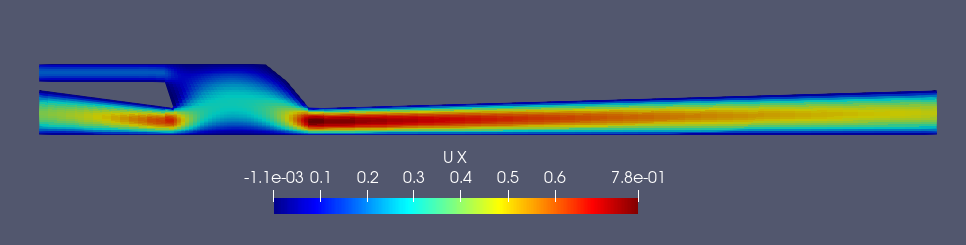
\includegraphics[width=1\textwidth]{Figuras/00_caso_intro.png}
    \end{figure}
    \bigskip\bigskip
    {\Huge Resumen:\\}
    Preparación de un caso para estudio RTD (Residence Time Distribution) con \textit{OpenFOAM}. 
    Definición de la malla con \textit{blockMesh} y simulación con solvers \textit{simpleFoam} (obtención campo de velocidades) y \textit{scalarTransportFoam} (distribución del campo escalar).
    
    \vspace*{\fill}
    Autor: Guillermo Rolle\par
    Supervisor: Dr. Ing. César Pairetti\par
    \bigskip
    Diciembre 2019
\end{center}
\end{titlepage}

%\maketitle
\tableofcontents
\newpage

\section{Introducción}
El objetivo de este trabajo es estudiar la calidad de mezclado en el tubo de salida de dos fluidos diferentes. En particular, en este trabajo se pensó un dispositivo de mezcla de agroquímicos en línea. Es decir, que la mezcla se realice en el momento en que se requiere en lugar de mezclar la cantidad suficiente de productos previo a salir al campo. \par
El problema de la técnica convencional radica en que la mezcla no es almacenable en depósito para un posterior uso obligándola a ser tratada adecuadamente para reducir la contaminación generada por estos químicos.\par
Los casos de simulación acá presentados se encuentran en el repositorio  \href{https://github.com/guillerolle/casos_cfd}{https://github.com/guillerolle/casos\_cfd}. Descargar o clonar repositorio para obtener los archivos necesarios para las simulaciones.\par
Nota: los resultados de las simulaciones no se incluyen en el repositorio para evitar consumir espacio en el mismo. Sólo se encuentran los diccionarios y archivos importantes para realizar las simulaciones. Las simulaciones corren a cuenta de cada uno.

\subsection{Información preliminar del problema}

\begin{figure}[h!]
\centering
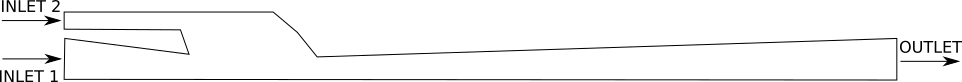
\includegraphics[width=1\textwidth]{Figuras/01_preliminar.png}
\caption{Geometría del problema}
\label{fig:preliminar}
\end{figure}

El fluido principal (agua) ingresa a alta presión por la entrada 1 succionando el fluido secundario (agroquímico) que ingresa por la entrada 2. La homogeneidad de la mezcla se evaluará en la salida del dispositivo.\par
\bigskip
En este trabajo se supondrá que el agroquímico tiene las mismas propiedas que el agua (densidad y viscosidad). De esta manera, se realizará una simulación para obtener el campo de velocidades para un único fluido en ambas entradas.\par
Luego, a partir del campo obtenido en estado estacionario, se hará otra simulación para estudiar la difusión y convección de un parámetro escalar que en este caso representará la concentración de agroquímico en cada punto del dominio de la simulación. Un valor de 1 indicará que el fluido es 100\% agroquímico en ese punto y un valor de 0 indicará que es 100\% agua (0\% agroquímico).

\subsection{Preparación del caso}
Copiaremos un caso de los tutoriales para preparar el nuestro a partir de ese. Una vez abierta una terminal y 
cargado el ambiente de OpenFOAM, ejecutar:
\marginnote{\small \textbf{Linux tips:\\} El símbolo '.' representa el directorio actual}
\begin{lstlisting}
$ run
$ mkdir 01
$ cp -r $FOAM_TUTORIALS/incompressible/simpleFoam/pitzDaily ./01
$ cd 01
\end{lstlisting}

En la carpeta de nuestro caso \textit{01\_rtd} tendremos
la siguiente estructura de archivos:\par

\begin{lstlisting}
01
|-- 0
|   |-- epsilon
|   |-- f
|   |-- k
|   |-- nut
|   |-- nuTilda
|   |-- omega
|   |-- p
|   |-- U
|   `-- v2
|-- constant
|   |-- transportProperties
|   `-- turbulenceProperties
`-- system
    |-- blockMeshDict
    |-- controlDict
    |-- fvSchemes
    |-- fvSolution
    `-- streamlines.

3 directories, 16 files
\end{lstlisting}


\marginnote{\small \textbf{Linux tips:\\} \textit{man cmd} muestra el manual del comando \textit{cmd}. Por ejemplo, \textit{man cd}}
En primer lugar, la simulación que vamos a realizar es laminar por lo que tendremos que modificar las propiedades de turbulencia. Abrir\\ \texttt{constant/turbulenceProperties} con el editor de textos de preferencia y eliminaremos los archivos \texttt{0/epsilon, 0/f, 0/k, 0/nut, 0/nuTilda, 0/omega, 0/v2}. Por ejemplo:\par
\begin{lstlisting}
$ cd 0
$ rm epsilon f k nut nuTilda omega v2
$ cd ../constant
$ nano turbulenceProperties
[...]
simulationType laminar; <- MODIFICAR ESTA LINEA
[...]
\end{lstlisting}
\marginnote{\small \textbf{Linux tips:\\} '..' representa el directorio superior}

\noindent Ver archivo completo: \href{https://github.com/guillerolle/casos_cfd/blob/master/01/constant/turbulenceProperties}{constant/turbulenceProperties}
%\lstinputlisting[caption=\textit{constant/turbulenceProperties},frame=shadowbox]{OpenFOAM/turbulenceProperties.txt}

\section{Mallado}
Se utilizará el mallador \textit{\href{https://cfd.direct/openfoam/user-guide/v6-blockmesh/}{blockMesh}} de OpenFOAM. En la figura \ref{fig:blockMesh} se puede ver la disposición de los vértices y bloques para crear el archivo \textit{blockMeshDict}.

\begin{landscape}
\newpage
%\KOMAoptions{paper=landscape,pagesize}
%\recalctypearea
	\begin{figure}[h!]
	\centering
	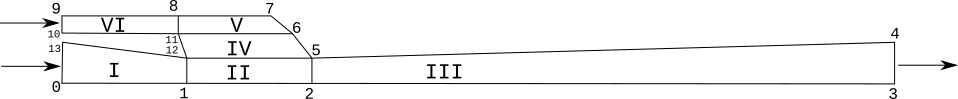
\includegraphics[width=1.5\textheight]{Figuras/01_blockMesh.png}
	\caption{Vértices y bloques para blockMesh}
	\label{fig:blockMesh}
	\end{figure}
\bigskip
	\begin{figure}[h!]
	\centering
	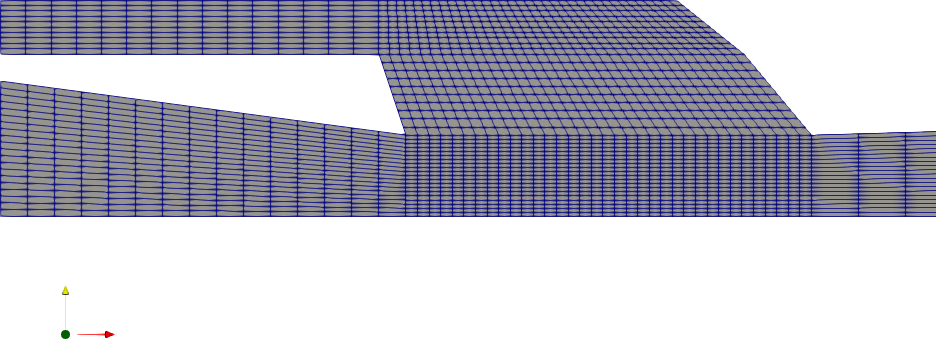
\includegraphics[width=1.5\textheight]{Figuras/01_mallado.png}
	\caption{Malla creada con blockMesh (zoom)}
	\label{fig:malla}
	\end{figure}
\end{landscape}
	
%\marginnote{\small \textbf{OpenFOAM tips:\\} Es posible definir parámetros de la forma\\ \textit{param valor;} y llamarlos con \textit{\$param}}
%\lstinputlisting[caption=\textit{system/blockMeshDict},frame=shadowbox]{OpenFOAM/blockMeshDict.txt}
\noindent Ver archivo completo: \href{https://github.com/guillerolle/casos_cfd/blob/master/01/system/blockMeshDict}{system/blockMeshDict}

\bigskip\bigskip
\marginnote{\small \textbf{Linux tips:\\} \textit{touch <file>} crea un archivo vacío con el nombre \textit{<file>}}
Una vez definido el archivo \textit{system/blockMeshDict} ejecutar los siguientes comandos para crear la malla con \textit{blockMesh}:
%\begin{wrapfigure}{R}{0.4\linewidth}
%\begin{bclogo}[couleur = blue!30,arrondi = 0.1, ombre = true]{OpenFOAM tips}
%El comando checkMesh permite revisar entre otras cosas la ortogonalidad del mallado.
%\end{bclogo}
%\end{wrapfigure}
\begin{lstlisting}
$ blockMesh
\end{lstlisting}
\bigskip
Si el comando se ejecuta correctamente podemos mirar la malla en \textit{ParaView} (\ref{fig:malla}). Observar la ortoganilidad de la malla. 

\marginnote{\small \textbf{Linux tips:\\} El símbolo \& al final de la línea permite seguir utilizando la terminal actual}
\begin{lstlisting}
$ touch rtd.foam 
$ paraview rtd.foam &
\end{lstlisting}

O, equivalentemente:

\begin{lstlisting}
$ paraFoam 
\end{lstlisting}
\bigskip
\marginnote{\small \textbf{OpenFOAM tips:\\} El comando \textit{paraFoam} ejecuta esencialmente los dos comandos  anteriores para abrir ParaView}

Antes de continuar con el caso es conveniente observar la salida del comando \textit{\href{https://openfoamwiki.net/index.php/CheckMesh}{checkMesh}} para comprobar la calidad del mallado. Por ejemplo, una malla "no-ortogonal" puede resultar en fallas en la resolución numérica del caso. Ver el siguiente documento sobre \href{http://www.wolfdynamics.com/wiki/meshing_preliminaries_and_quality_assessment.pdf}{calidad de mallado}.
\begin{lstlisting}
$ checkMesh
[...]
Checking geometry...
    Overall domain bounding box (0 0 -0.001) (0.1 0.008 0)
    Mesh has 2 geometric (non-empty/wedge) directions (1 1 0)
    Mesh has 2 solution (non-empty) directions (1 1 0)
    All edges aligned with or perpendicular to non-empty directions.
    Boundary openness (7.19353e-18 -4.50911e-17 -3.44031e-15) OK.
    Max cell openness = 2.13343e-16 OK.
    Max aspect ratio = 11.4754 OK.
    Minimum face area = 6.35714e-08. Maximum face area = 1.75071e-06.  Face area magnitudes OK.
    Min volume = 6.35714e-11. Max volume = 4.35313e-10.  Total volume = 4.8025e-07.  Cell volumes OK.
    Mesh non-orthogonality Max: 50.9374 average: 16.2357 <- CUANTO MAS ALTO EL VALOR MAXIMO DE NO-ORTOGONALIDAD, MAYORES SERAN LOS ERRORES NUMERICOS DEBIDOS LA MALLA!!
    Non-orthogonality check OK.
    Face pyramids OK.
    Max skewness = 0.928968 OK.
    Coupled point location match (average 0) OK.

Mesh OK.

End

\end{lstlisting}

\section{Preparación de la simulación}
Después de crear la malla hay que ajustar los archivos \texttt{0/U}, \texttt{0/p},\\ \texttt{system/fvSchemes}, \texttt{system/fvSolutions} y \texttt{system/controlDict}.

\subsection{Condiciones iniciales}
El campo de velocidades podemos definirlo como nulo en todo el dominio porque impondremos condiciones de presión. En las entradas y salidas utilizamos la condición \textit{\href{https://www.cfdsupport.com/OpenFOAM-Training-by-CFD-Support/node113.html}{zeroGradient}}. 

Ver archivo completo de condición inicial de velocidad: \href{https://github.com/guillerolle/casos_cfd/blob/master/01/0/U}{0/U}

%\newpage
%\marginnote{\small \textbf{OpenFOAM tips:\\} Una línea comenzando con // es un comentario y el sofware lo ignorará}
%\lstinputlisting[caption=\textit{0/U},frame=shadowbox]{OpenFOAM/U.txt}
\bigskip
En cuanto a las presiones, impondremos 300MPa en la entrada de agua y un valor de 0 en la salida. En la entrada de agroquímico nos interesa que la presión sea mayor que la presión del agua en el empalme de los tubos. De esta manera permitiría al agroquímico a ser succionado por el flujo de agua.\par
Gracias a la tobera en la entrada, existe una depresión en la zona de unión. Impondremos un valor de 300MPa para asegurarnos que la presión sea mayor en ese lugar.

Ver archivo completo de condición inicial de presión: \href{https://github.com/guillerolle/casos_cfd/blob/master/01/0/p}{0/p}
%\lstinputlisting[caption=\textit{0/p},frame=shadowbox]{OpenFOAM/p.txt}

\subsection{Diccionarios en system}
Estos diccionarios contienen información sobre los solvers, pasos de tiempo, métodos numéricos, etc.
El más importante es \href{https://github.com/guillerolle/casos_cfd/blob/master/01/system/controlDict}{system/controlDict}. Cabe destacar que \textit{simpleFoam} es un solver estacionario, así que lo que se define como tiempo en este diccionario, es en realidad un número que se le asigna a cada iteración. Se pone un deltaT igual a 1 para facilitar la lectura de los archivos generados.
\begin{lstlisting}
[...]
deltaT 	  1;  // Solamente sirve para enumerar las iteraciones. No afecta a la simulacion
[...]
\end{lstlisting}

Los otros dos contienen información sobre los esquemas numéricos y tolerancias.\par
Ver archivo: \href{https://github.com/guillerolle/casos_cfd/blob/master/01/system/fvSchemes}{system/fvSchemes}\par
Ver archivo:
\href{https://github.com/guillerolle/casos_cfd/blob/master/01/system/fvSolution}{system/fvSolution}
%\lstinputlisting[caption=\textit{0/p},frame=shadowbox]{OpenFOAM/p.txt}



%\lstinputlisting[caption=\textit{system/controlDict},frame=shadowbox]{OpenFOAM/controlDict.txt}
%\lstinputlisting[caption=\textit{system/fvSchemes},frame=shadowbox]{OpenFOAM/fvSchemes.txt}
%\lstinputlisting[caption=\textit{system/fvSolution},frame=shadowbox]{OpenFOAM/fvSolution.txt}

%\newpage
\section{Simulación: \textit{\href{https://openfoamwiki.net/index.php/SimpleFoam}{simpleFoam}}}
\marginnote{\small \textbf{Linux tips:\\} El símbolo $|$ toma la salida del primer comando (izquierda) y la usa como entrada del segundo (derecha)}
Ahora estamos listos para ejecutar la simulación primer simulación para obtener el campo de velocidades en el dispositivo. En el directorio principal del caso:

\begin{lstlisting}
$ simpleFoam | tee log
\end{lstlisting}


Si todo se ejecuta correctamente podremos abrirlo con ParaView (o clickear en 'reload' si ya está abierto):
\begin{lstlisting}
$ paraview rtd.foam &
\end{lstlisting}

\marginnote{\small \textbf{Linux tips:\\} El comando \textit{tee file} guarda lo que recibe como entrada en el archivo \textit{file}. Ver \textit{man tee}}
\begin{figure}[h!]
\centering
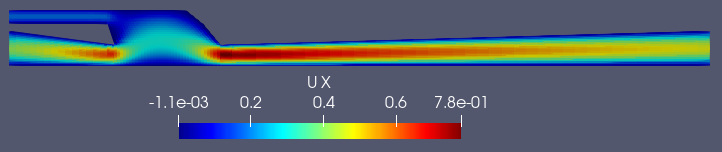
\includegraphics[width=1\textwidth]{Figuras/campo_vel.png}
\caption{Campo de velocidad}
\label{fig:campo_vel}
\end{figure}

En este caso nos interesaría saber si el flujo de agroquímico efectivamente es expulsado por el tubo de salida. Podemos comprobar esto, sabiendo que la simulación es laminar, con un filtro en ParaView. Presionar
\texttt{Ctrl + Space} y buscar el filtro \textit{StreamTracer}. Podemos ubicar el filtro alineado con el eje Y en el tubo de salida y mostraremos unas 50 líneas de traza.

\begin{figure}[h!]
\centering
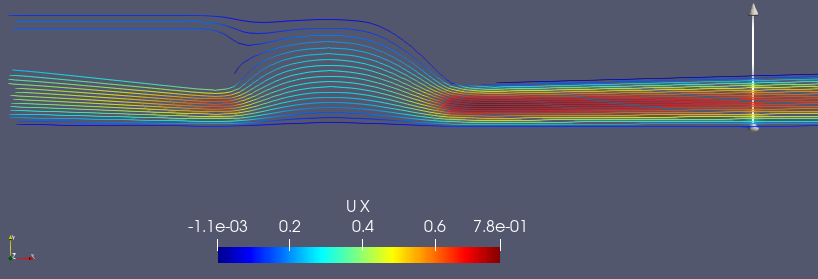
\includegraphics[width=1\textwidth]{Figuras/stream_vel.png}
\caption{Líneas de traza}
\label{fig:stream_vel}
\end{figure}

Las líneas de traza correspondientes al tubo superior indican que, efectivamente, el agroquímico es succionado en el dispositvo. 

Podemos cargar el archivo de estado de ParaView \textit{rtd\_pU.pvsm} y nos abrirá el entorno de ParaView con las gráficas y filtros correspondientes. La simulación debe estar realizada anteriormente.

\section{Preparación del caso RTD}
Como base para la simulación del transporte escalar copiaremos otro de los tutoriales en una carpeta nueva. En la carpeta principal del caso:
\begin{lstlisting}
$ mkdir RTD
$ cp -r $FOAM_TUTORIALS/basic/scalarTransportFoam/pitzDaily ./RTD
$ cd RTD
\end{lstlisting}

Tendremos la siguiente estructura de archivos:
\begin{lstlisting}
RTD
|-- 0
|   |-- T
|   `-- U
|-- constant
|   `-- transportProperties
`-- system
    |-- blockMeshDict
    |-- controlDict
    |-- fvSchemes
    `-- fvSolution

3 directories, 7 files
\end{lstlisting}

Copiamos la malla del caso anterior en el caso RTD.
\begin{lstlisting}
$ cp -r ../constant/polyMesh ./constant
\end{lstlisting}

Como antes, podemos comprobar que la malla esté creada correctamente ejecutando
\begin{lstlisting}
$ paraFoam
\end{lstlisting}

\subsection{Condiciones iniciales}
Para el campo de velocidad usaremos el obtenido en la simulación anterior. En este caso, la última iteración es la 110. Por lo tanto

\begin{lstlisting}
$ cp ../110/U ./0
\end{lstlisting}

La concentración de agroquímico será representada en este caso por la variable \textit{T}. Un valor de 1 indicaría que el fluido es agroquímico puro y un valor de 0 indicaría que el fluido en ese lugar es únicamente agua.

Entonces, para el \textit{inlet\_one} pondremos una condición tipo \textit{fixedValue} con valor 0 y para \textit{inlet\_two} un valor de 1. Para el \textit{outlet} pondremos condición \textit{zeroGradient}.

Por ejemplo, para \textit{inlet\_one}:
\begin{lstlisting}
inlet_one 
{
	type	fixedValue;
	value	uniform 0;
}
\end{lstlisting}

Ver el archivo completo: \textit{\href{https://github.com/guillerolle/casos_cfd/blob/master/01/RTD/0/T}{RTD/0/T}}

%\lstinputlisting[caption=\textit{RTD/0/T},frame=shadowbox]{OpenFOAM/T.txt}

\subsection{Propiedades del fluido}
En la carpeta \textit{constant} debemos definir un valor para el coeficiente de difusión del agroquímico. Propondremos un valor de 0.00005 (ojo! corroborar con el repositorio el valor más actualizado):

\bigskip\bigskip

\marginnote{\small \textbf{OpenFOAM tips:\\} En la versión \textit{\href{https://openfoam.org/}{dev}} es necesario definir las unidades de la difusividad mientras que en la  \textit{\href{https://openfoam.com/}{plus}} no.}
\begin{lstlisting}
...
DT                         0.00005; // Para OpenFOAM-plus (v1906)
DT   DT [0 2 -1 0 0 0 0] 0.00005; // Para OpenFOAM-dev (7)
...
\end{lstlisting}

Ver el archivo completo: \textit{\href{https://github.com/guillerolle/casos_cfd/blob/master/01/RTD/constant/transportProperties}{RTD/constant/transportProperties}}

%\lstinputlisting[caption=\textit{RTD/constant/transportProperties},frame=shadowbox]{OpenFOAM/RTD/transportProperties.txt}


\subsection{Diccionarios en \textit{system}}
Nuevamente, estos diccionarios contienen información sobre los solvers, pasos de tiempo, métodos numéricos, etc.
El más importante es \textit{\href{https://github.com/guillerolle/casos_cfd/blob/master/01/RTD/system/controlDict}{RTD/system/controlDict}}.  Esta vez, como el solver \textit{scalarTransportFoam} es un solver transitorio, las variables de tiempo sí representan tiempos y no iteraciones.

\begin{lstlisting}
...
endTime 2; // en segundos ambas. Chequear ultima version en repositorio
deltaT 	  0.001;  
...
\end{lstlisting}

Los otros dos contienen información sobre los esquemas numéricos y tolerancias.\par
Ver archivo: \textit{\href{https://github.com/guillerolle/casos_cfd/blob/master/01/RTD/system/fvSchemes}{RTD/system/fvSchemes}}\par
Ver archivo:
\textit{\href{https://github.com/guillerolle/casos_cfd/blob/master/01/RTD/system/fvSolution}{RTD/system/fvSolution}}


%\lstinputlisting[caption=\textit{RTD/system/controlDict},frame=shadowbox]{OpenFOAM/RTD/controlDict.txt}
%\lstinputlisting[caption=\textit{RTD/system/fvSchemes},frame=shadowbox]{OpenFOAM/RTD/fvSchemes.txt}
%\lstinputlisting[caption=\textit{RTD/system/fvSolution},frame=shadowbox]{OpenFOAM/RTD/fvSolution.txt}

\section{Simulación: \textit{scalarTransportFoam}}
Ya tenemos el caso RTD preparado y podemos ejecutar la simulación con el solver \textit{scalarTransportFoam}. Cabe destacar que este es un solver transitorio a diferencia de \textit{simpleFoam} que es estacionario.

\begin{lstlisting}
$ scalarTransportFoam | tee log
$ paraFoam
\end{lstlisting}

Podemos cargar el archivo de estado de ParaView \textit{RTD.pvsm} para abrir las gráficas y filtros correspondientes.

\begin{figure}[h!]
	\centering
	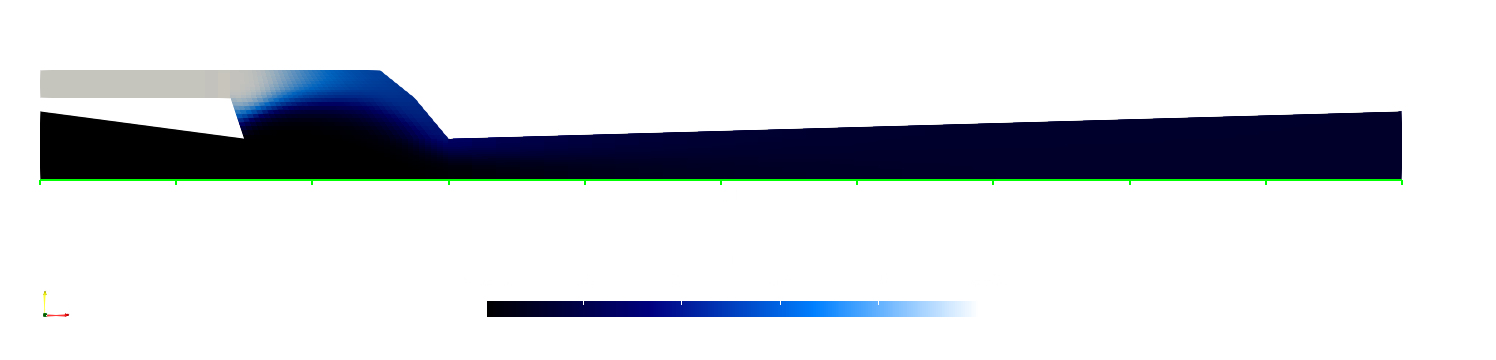
\includegraphics[width=1\textwidth]{Figuras/campo_T.png}
	\caption{Concentración de agroquímico (t = 2s)}
	\label{fig:campo_t}
\end{figure}

\newpage
\section{Post proceso}
Nos interesa conocer la concentración promedio en toda el área de salida del dispositivo. En la carpeta \textit{system} del caso RTD copiaremos el archivo \textit{patchAverage} de la carpeta \textit{etc} de OpenFOAM. En la carpeta principal RTD ejecutar:

\begin{lstlisting}
$ cp $FOAM_ETC/caseDicts/postProcessing/surfaceFieldValue/patchAverage ./system
$ nano system/patchAverage
\end{lstlisting}

En este archivo debemos modificar los campos \textit{patchName} y \textit{field names} con nuestros valores de interés. Los cambios son los siguientes:
\begin{lstlisting}
...
name  outlet;
fields (T);
...
\end{lstlisting}

\noindent Ver el archivo completo: 
\href{https://github.com/guillerolle/casos_cfd/blob/master/01/RTD/system/patchAverage}{RTD/system/patchAverage}
\bigskip

%\lstinputlisting[caption=\textit{RTD/system/patchAverage},frame=shadowbox]{OpenFOAM/RTD/patchAverage.txt}

Podemos ejecutar el post-proceso con el siguiente comando.

\begin{lstlisting}
$ postProcess -func 'patchAverage'
\end{lstlisting}

Esto nos va a crear una carpeta \textit{postProcessing/patchAverage/0} con el archivo \textit{surfaceFieldValue\_0.dat}. Cambiamos de directorio para analizar más fácilmente estos datos:
\begin{lstlisting}
$ cd postProcessing/patchAverage/0
\end{lstlisting}

Ese archivo contiene el valor de areaAverage(T) para cada instante de tiempo dispuestos en columna. Para ver el contenido del archivo en la terminal ejecutar:
\begin{lstlisting}
$ cat surfaceFieldValue_0.dat
\end{lstlisting}

Este archivo podemos leerlo directamente en \textit{gnuplot} para realizar una gráfica de la concentración en función del tiempo.

\begin{lstlisting}
$ gnuplot
gnuplot> plot 'surfaceFieldValue\_0.dat' w l title "outlet"
gnuplot> set xlabel "Tiempo [s]"
gnuplot> set ylabel "Concentracion []"
gnuplot> replot
\end{lstlisting}

Observamos que la concentración en la salida converge a un valor de aproximadamente 15\%.

\newpage
\begin{figure}[h!]
\centering
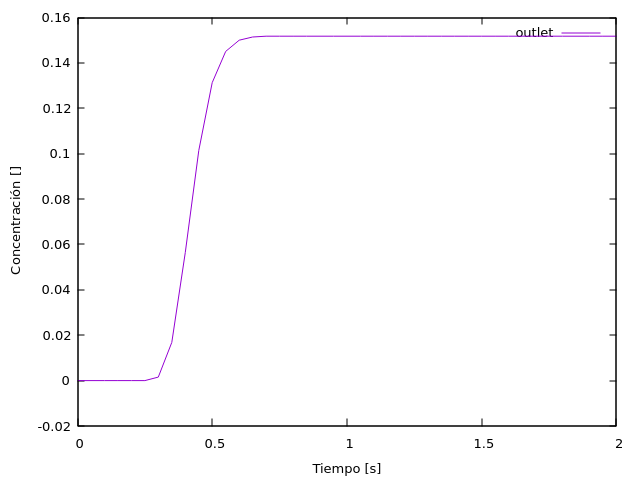
\includegraphics[width=1\textwidth]{Figuras/curva_concentracion.png}
\caption{Concentración en la salida en función del tiempo}
\label{fig:curva_conc}
\end{figure}

Podemos también observar el perfil de concentración sobre la salida para comprobar la homogeneidad de la mezcla. Esto se ve en rojo en la figura \ref{fig:curvas_outlet}.

\begin{figure}[h!]
	\centering
	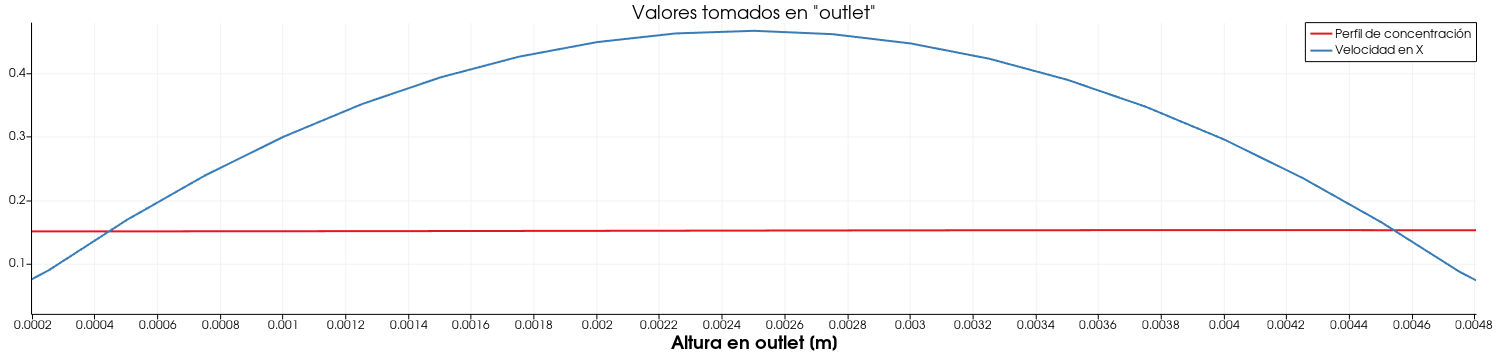
\includegraphics[width=1\textwidth]{Figuras/outlet_graficas.png}
	\caption{Distribución de valores sobre toda la altura del outlet}
	\label{fig:curvas_outlet}
\end{figure}

%\newpage
%#\bibliographystyle{plain}
%#\bibliography{references}
\end{document}
